\documentclass[12pt,twocolumn]{article}
\usepackage{fancyhdr}
\usepackage{extramarks}
\usepackage{amsmath}
\usepackage{amsthm}
\usepackage{amsfonts}
\usepackage{tikz}
\usepackage[plain]{algorithm}
\usepackage{algpseudocode}
\usepackage{hyperref}
\usepackage[utf8]{inputenc}
\usepackage[english]{babel}

\setlength{\parindent}{0cm}
% \addtolength{\oddsidemargin}{-2cm}
% \addtolength{\evensidemargin}{-2cm}
% \setlength{\textwidth}{17.78cm}
\addtolength{\topmargin}{-2.25cm}
\setlength{\textheight}{24.24cm}
\addtolength{\parskip}{5mm}

\pagestyle{fancy}

% \renewcommand\headrulewidth{0.4pt}
\renewcommand\footrulewidth{0.4pt}

\setlength\parindent{0pt}



\DeclareMathOperator*{\argmax}{arg\max}


\title{Exploring the effects of different reward functions on the TSCA learning process}
\author{Drew Kristensen\\McGill ID: 260923149}
\begin{document}
\maketitle

\begin{abstract}
While there has been extensive research into the applications of reinforcement learning with controlling a traffic signal control agent (TSCA), there has been little comparison between the reward functions used by different approaches. In this paper, we explore 6 different reward functions, each measured once with the current time step, and once as a difference with the previous time step, all standardized by using the same model, action space, and state space.
\end{abstract}

\section{Introduction}
%Motivation
Traffic congestion is a problem that most people in urban environments have experienced at some point in their lives. Congestion not only has an impact on the humans involved in the traffic jam, but the idling vehicles emitting carbon cause environmental harm.
It is estimated that in 2013, the annual time wasted in cities due to congested traffic was around 65 hours per driver, and the amount of carbon dioxide released while delayed was approximately 3.1 megatons per major city \cite{CEBR}.
The factors responsible for this traffic congestion can be attributed to a few sources, namely the increase in the number of vehicles on the road, inadequate infrastructure, and inefficient current intersection controls.
To alleviate congestion, at least one of the above reasons must be addressed.
Since construction of new infrastructure in urban environments is costly, and since cars will continue to be driven, the most realistic solution involves utilizing a smarter traffic controller.
%Explanation of TSCA
The most basic traffic controllers use fixed time signal control, where the timings of the lights can be fitted to data in order to optimize throughput.
The problem with fixed timing controls is that it cannot react to real-world changes in traffic throughput, and can lead to congestion and gridlock in urban environments. 
Currently, an effective solution to reducing vehicular congestion is using adaptive traffic signal control, where the timings on light signals are changed according to real world data that the traffic signal control agent (TSCA) can collect.
Current examples of these include SCOOT and TRANSYT \cite{Robertson1991} and prove to be much more effective than their static equivalent, however, the extensive work into reinforcement learning (RL) applications to TSCAs have shown great prospect, and large reductions in delays compared to these improved dynamic signals.
% 
%Explanation of Q-learning
We implement the Q learning algorithm with experience replay \cite{Watkins1989, DeepmindAtari, DeepmindLocomotion}. Q learning is the process of training an approximator to estimate a Q function, where the Q function represents
\[
    Q(s_t,a_t,\pi) = \mathbb{E}\left\{\sum_{k=0}^{\infty}\gamma^kr_{t+k}\middle| s_t,a_t,\pi\right\}
\]

for a given state (\(s_t\)) and action (\(a_t\)), taken under some policy \(\pi\). That is, the Q function outputs the expected value of all rewards from the current action and state onwards. The discount factor, \(\gamma\), is a value between 0 and 1, and is used to weight the actions taken now and in the near future more heavily than the rewards from actions take in the distant future. By operating on the rewards, we can choose an action at time \(t\) with
\[
    a_t = \argmax_{a}Q(s_t,a,\pi)
\]
.
The goal of Q learning is to find some policy \(\pi^*\) such that \(\pi^* = \argmax_{\pi}Q(s,a,\pi)\), for all \(s\in S, a\in A\).

We train towards this policy by the iterative value update defined by setting 
\[
    Q(s_t,a_t,\theta) \leftarrow r_t+\max_{a\in A}Q(s_{t+1},a,\theta)
\]
Where \(\theta\) is the parameters for our network.

\section{Related Works}

As the idea of applying reinforcement learning to the TSCA problem is not new \cite{Thorpe}, there has been many projects exploring novel state and action spaces, yet only a few of the possible reward functions have been explored. This is because choosing the \emph{best} reward function is an unsolved problem in reinforcement learning, and the best approach in the past has been trial and error. In Brys et al \cite{Brys2014}, the authors compared using delay, squared delay, and throughput as reward functions for a RL TSCA, but these reward functions were more used to compare the differences between algorithms. Genders and Razavi \cite{Genders} chose to use the change in cumulative vehicle delay for their experiments, a reward function that we test in this study due to the success of their model in reducing not only cumulative delay, but increasing throughput and decreasing queues. Chu et al. \cite{Chu} used a combination of two common reward functions for their Multi Agent RL TSCA, namely a linear combination of the queue length and the wait time at each time step. Until this point, there had not been multi-reward reward functions utilized in the TSCA, and their model proved to be successful by their metrics, including queue length and average delays. One of the more extensive and novel evaluations of reward functions comes from the PhD thesis of Tantawy \cite{Tantawy}, where they examine change in delay, maximizing reduction of cumulative delay, and minimization/balancing of queue length. While all of these experiments show the variety of reward functions, there is no way to compare the effects of the individual reward functions compared to one another.

\section{Method}

\subsection{State Space}
The state space we use in this experiment is the Discrete Traffic State Encoding (DTSE) developed by Genders and Razavi in 2016 \cite{Genders} as an efficient way to encode the information of a controlled intersection in a concise manner. The DTSE works by discretizing the lanes into cells of length \(c\), giving us \(\frac{l}{c}\) cells, where \(l\) is the length of our lanes. We split the information of the junction into three parts; the first for the current traffic signal, the second for the presence of vehicles in cells, and the third for the speed of vehicles in the cell relative to the speed limit. An example can be seen in figure \ref{fig:DTSE_Genders}, but this lacks some clarity so see section \ref{sec:DTSE_explanation} for a more in-depth explanation.

\begin{figure}
    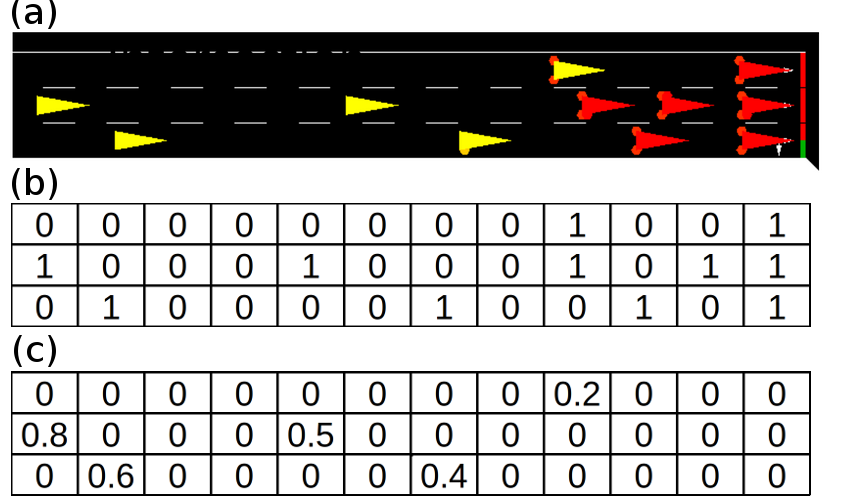
\includegraphics[height=0.2\textheight]{Figures/dtse_example}
    \caption{DTSE example from Genders, Razavi 2016}
    \label{fig:DTSE_Genders}
\end{figure}

\subsection{Action Space}
The action space for this experiment is also taken from Genders and Razavi's 2016 paper \cite{Genders}, as it provides a moderate level of freedom for our TSCA. This is ideal for this experiment as giving it too much freedom, as we could by allowing our TSCA to choose the signal at each time step without forcing any structure on the transitions, increases the amount of training needed to achieve a policy that prevents collisions in our junction at each time step, much less performs well. However, if we restrict the freedom of the TSCA too much, then we end up with something much more akin to today's standard timed lights. Finding a perfect medium is an ongoing effort, however the Genders action space is intuitive and easy to implement. In short, we simply force a short transition period between any two differing green light signals. We can think of a four way intersection, such as the one used in our experiments, as having only 4 signals. One for North-South traffic allowed to move forward through the intersection, and yield on left turns, one for North-South traffic allowed to make protected left turns, and two equivalent signals for East-West traffic. We don't need to include red light signals this way, as we can simply think of them as the green counterparts for the opposing direction. By using Genders and Razavi's action space, we force each of these 4 signals to interject a transitional period of yellow lights when changing from one to another. An example of this schedule can be seen in figure \ref{fig:action_transitions}. However, with our implementation, we add two all-yellow signals to each direction, as a way to bridge between from all-green signals from one direction to a signal in the opposing direction. This gives us an easy way to safely slow down the traffic, without needing to learn the dynamics of a traffic system with the actions space with large amounts of freedom.

\begin{figure}
    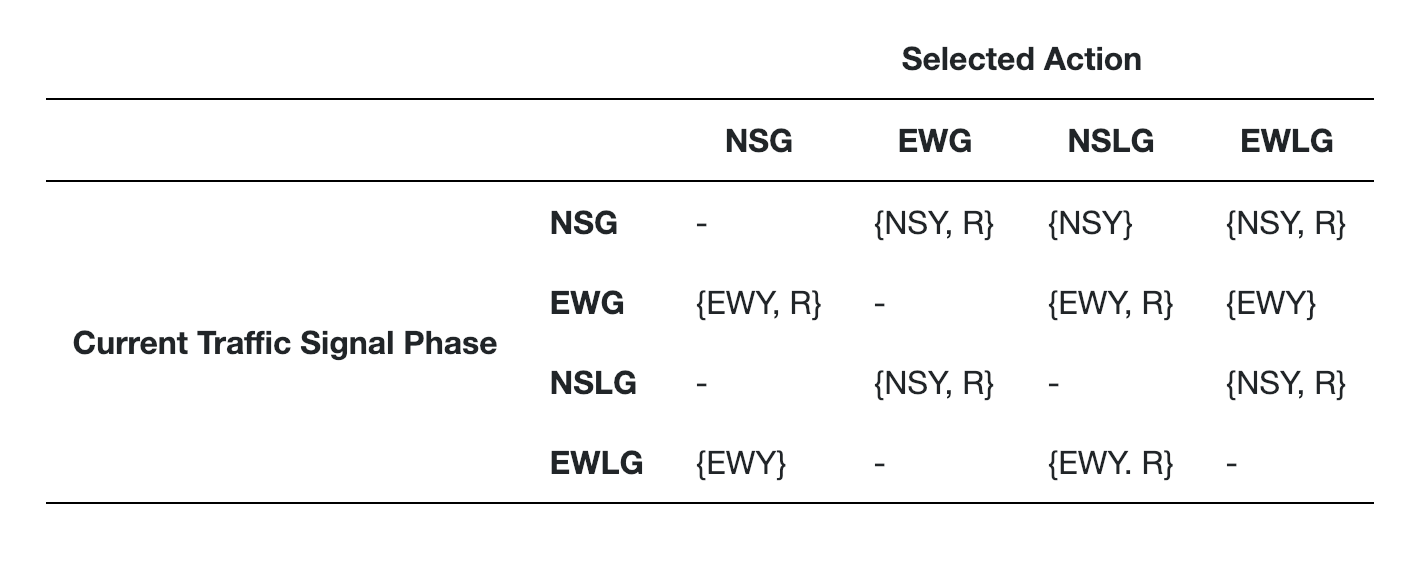
\includegraphics[width=0.4\textwidth]{Figures/genders_actions}  
    \caption{Action transition map from Genders, Razavi 2016}
    \label{fig:action_transitions}
\end{figure}

\subsection{Reward Functions}
As the topic of this paper's exploration, we have 12 reward functions with which we would have liked to test. The first 6 are simply each reward function at each time step, while the latter 6 are the same reward functions, only altered by subtracting the reward at the current time step from the reward from the previous time step. That is, our base reward \(R_t(s_{t},a_{t}))\) is a function of only the previous state and action, whereas our augmented rewards (the latter 6 of our given rewards) can be written as \(R_t^{'}(s_{t-1},a_{t-1},s_t,a_t) = R_{t-1}(s_{t-1},a_{t-1}) - R_t(s_{t},a_{t})\). The goal of including both of these types of rewards is to investigate the presence or absence of a benefit from using a reward function that uses more than just one time step's worth of information.

\subsubsection{Queue Length}
The first of our reward functions is the queue length. This is one of the simplest and earliest metrics used for the TSCA problem with RL, as it is an intuitive metric to be minimizing. In order to compute this metric, we simply take the sum the number of cars stopped at the light in each lane across all lanes controlled by the TSCA. This is a natural reward function to start with, as minimizing the amount of cars waiting at the light would intuitively move traffic through the intersection.

\subsubsection{Linear Delay}
Linear delay is another intuitive metric to use, as it simply measures the amount of time that each car is delayed in our network. To compute our values of linear delay, we sum the waiting time of each loaded vehicle in the network, such that the vehicle is not yet through the network and on its arrival lane. This value gives us our cumulative linear delay, and dividing by the number of applicable vehicles gives us our average linear delay. See section \ref{sec:delay_error} for notes on the problem with our implementation during our training window.

\subsubsection{Squared Delay}
Squared delay is a less explored metric than linear delay, but there are solid motivations to using it. Squared delay is computed in a similar fashion to the linear delay, except instead of summing the delays of each vehicle, we sum the squares of the delays of each vehicle. The intuition behind this approach is to limit the amount of time any individual driver spends waiting at the traffic light, even if it comes at a small cost to a number of other drivers. For example, if a small cross street has one driver attempting to cross a busy major street, linear delay would dictate that the single car on the cross street might need to wait upwards of 100 seconds in order to merit switching the signals for them to cross to compensate for the fact that the large volume of cross traffic will incur a large penalty. With squared delay, this problem is lessened, as the single car will quickly incur a larger penalty relative to what will be incurred from the short stop of the cross traffic. Again, see section \ref{sec:delay_error} for notes on the problem with our implementation during our training window.

\subsubsection{Average Arrived Travel Time}
Average arrived travel time (AATT) is another reward, which hasn't been explored in nearly the same depth as the first two. Typically used as a \emph{metric} and not as a \emph{reward}, average arrived travel time simply takes the average time it took for all cars which have arrived at their final destination, to travel from their starting destination to where they are. While this is a value that changes with the size of the network, that is, a network with edges of length 200 meters will undoubtedly have a longer average arrived travel time than that of a network with edge length of 100 meters, it still provides a valuable insight on how quickly cars are moving through this network. In our implementation, instead of taking the average travel time of \emph{all} arrived cars, we take the average travel time of the last 100 cars which arrived at their destination. This is a more near-sighted reward than the unlimited AATT, but we implemented it this way for memory constraints. 


\subsection{Model}
The model used in this exploration is a simple model comprised of only Linear layers, each followed by linear rectivation units as their associated non-linearity. The architecture can be seen in figure \ref{fig:model_architecture}. In order to train the model, we used the smooth L1 loss function implemented under Pytorch's functional module with the RMSProp optimizer with a learning rate of 2.5 e-4. We used a softmax exploration policy in order to explore unvisited state action pairs. Furthermore, we utilize an experience replay, which we initialize with 1000 random actions and their corresponding states from the simulation. This experience replay has a maximum capacity of 25,000 state, action, reward, and next state transition tuples.

\begin{figure}
    \begin{center}
    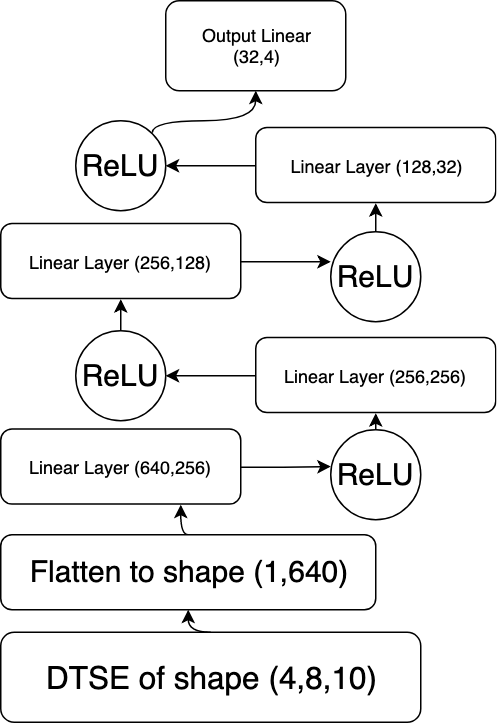
\includegraphics[height=.25\textheight]{Figures/model_architecture}
    \caption{Architecture of the model used}
    \label{fig:model_architecture}
    \end{center}
\end{figure}


\section{Results}

\subsection{Scenario}
The model and reward functions were trained and tested using the SUMO environment \cite{SUMO2018} with a 4 way intersection where each incoming road has 2 lanes. The leftmost lane for incoming traffic into the intersection was allowed either a left turn or a straight through the intersection, and the rightmost lane was allowed either a right turn or a straight trough. This intersection and its connections can be seen in figure \ref{fig:intersection_example}. Each incoming road had a length of 100 meters and a speed limit of 25 meters per second. Each training epoch consists of 2 hours of fairly heavy traffic with 1 car inserted into the simulation every 2 seconds, on average. Furthermore, as this is work done for a Canadian university, we used Canadian road laws in that no right hand turns were allowed under a red light. A simplification that we elected to make with our environment was to cut out pedestrian or cyclist traffic, simplifying the problem to only include vehicular traffic.

\begin{figure}
    \begin{center}
        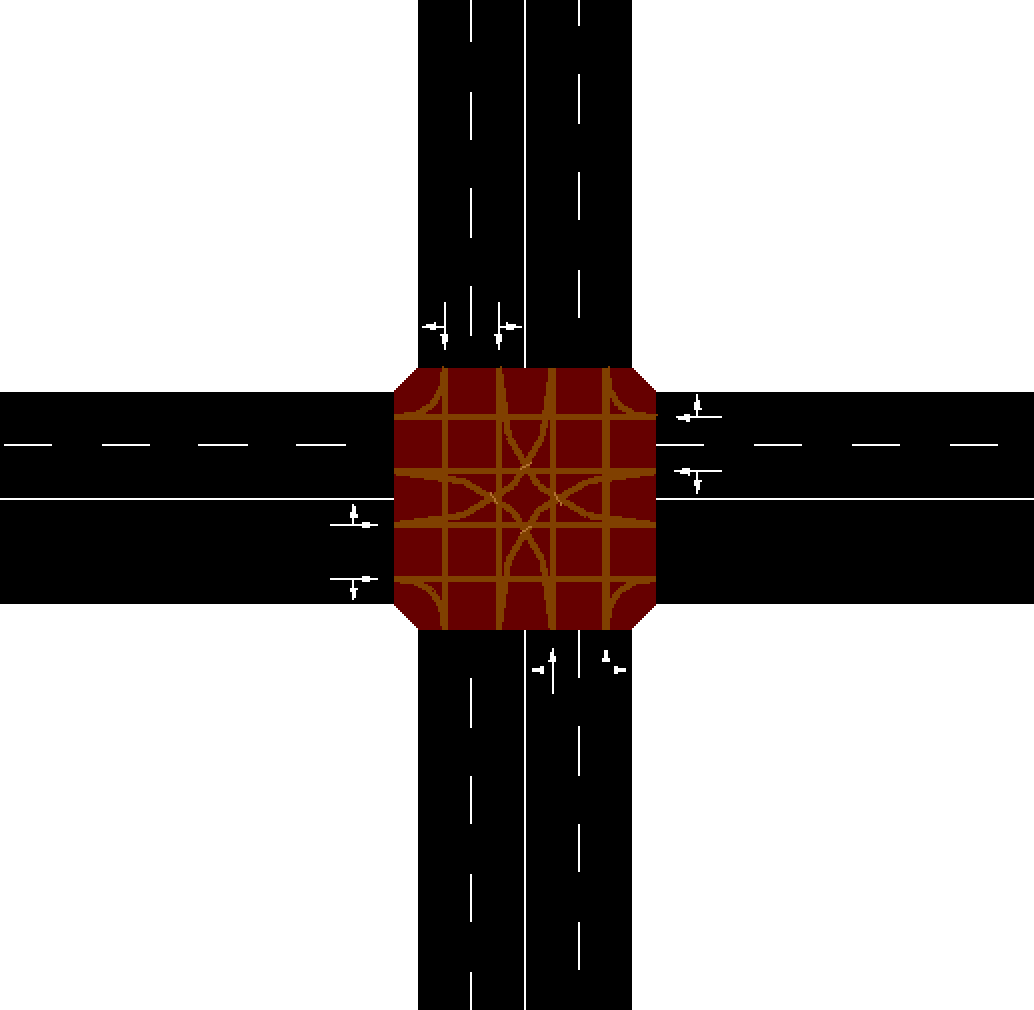
\includegraphics[height=0.25\textheight]{Figures/intersection_example}
        \caption{Intersection and underlying connections used in our simulation}
        \label{fig:intersection_example}
    \end{center}
\end{figure}

\subsection{Qualitative Results}

Due to constraints, both time and computational, we were only able to train using the first three reward functions out of the 12 total as well as only being able to train one single model, instead of the 5 we had wanted. This leads to extreme variance in what the true performance of the models trained using these reward functions are, and we are aware of this major issue. However, we were able to test these three models and measure their performance across all 12 rewards as well as measure their throughput. These tests were done in another heavy traffic environment for 40 simulated minutes. For the following graphs, blue shows the performance of the model trained using the queue length reward function, orange shows the model trained using the average linear delay, and green shows the model trained using the average squared delay.

To start, lets closely evaluate the results from figure \ref{fig:current_queue}, which shows the performance of the trained models evaluated using the average queue length. In order to understand this graph, it is important to know that our model could hold a maximum of up to 102 cars, so a network with an average queue length of 100 means that the lights never changed from red. Similarly, a network which never changes from a full green for one direction would have an average queue length of around 50. It is thus very evident that our squared delay agent was unable to change the lights from red to green for the first 100 or so epochs. I believe this in large part was due to the issue with the implementation, as the model was receiving a huge reward for flickering the green light and immediately changing back to the other direction. However, it can be seen that the queue length model consistently performed slightly better than leaving the green on for one direction the whole time, and all models seemed to be improving towards the end of the training. Again, with more training, we may have seen these become actually competitive with each other. 

\begin{figure}
    \begin{center}
    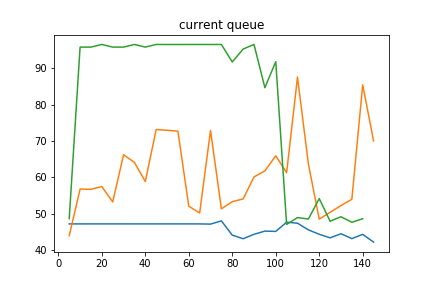
\includegraphics[width=0.45\textwidth]{Figures/current_queue}
    \caption{Performance of models tested on average queue length}
    \label{fig:current_queue}
    \end{center}
\end{figure}

Next, we can look at the results by comparing the average linear and squared delays. Due to the implementation error, the squared delay is simply the square of the linear delay, which it should not be, as the times should not reset by moving one space, leaving many of the squares to avoid exploding in value. In figure \ref{fig:current_avg_del}, we see that again the queue length model outperformed the other two models, and we see that the squared model was unable to learn anything significant about the task to lower its average delay.

\begin{figure}
    \begin{center}
    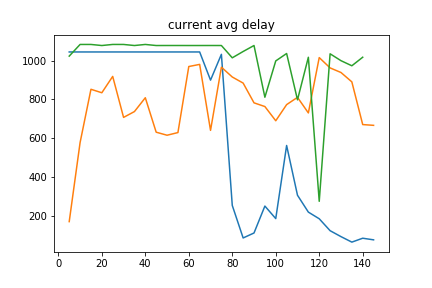
\includegraphics[width=0.45\textwidth]{Figures/current_avg_delay}
    \caption{Performance of models tested on average linear delay}
    \label{fig:current_avg_del}
    \end{center}
\end{figure}

For the full list of figures, see the figures folder in the code repository in section \ref{sec:github}.

\section{Conclusion}

In conclusion, we arrived at an unsatisfactory and insufficient conclusion given the flaws in the implementation before we detected them, our limited training window, and our limited computational power. As a solo project, the only computational tool available was a MacBook Pro, and the training window ended up being only about 24 hours once I had finished the implementation of all the parts of the code. However, despite all these shortcomings, we see that queue length out performed the mis-implemented delay rewards that we were able to train. 

\section{Appendix}

\subsection{Notable Error}
\label{sec:delay_error}

Due to an error in our code, we utilized a function from our simulator to compute the waiting times for the delays incorrectly. Thus, our waiting time per car only represents the time that car spent at a stop, not waiting at the light. For example, if a car is stopped a position 5 in the queue and accumulates 10 seconds of delay, if the light lets through even one of the cars in front of it in the queue, since the car will move forward one position, this resets the delay we measure back to 0, even though the vehicle is still delayed at the light. Due to time constraints, we were unable to rectify this error in our tests, only in our code. This is a major issue in our testing, as it does not accurately measure what we had hoped to measure and we believe it to be a major contributing factor to the dismal results. Even after this report is submitted, we will continue testing, and update our code repository with our results, as we ourselves are interested in achieving the correct information, even if there is no use for this report.

\subsection{DTSE Explanation}
\label{sec:DTSE_explanation}

We initialize our DTSE to be an array of zeros of shape 
\[
    DTSE(S_t) = [|A|, |L|, 2*\frac{\ell}{c}]
\] where \(A\) is our action space, \(L\) is the lanes controlled by the TSCA, \(\ell\) is the length of our lanes, and \(c\) is the cell length. Let us use our four action, action space. Let these actions be \{NSG, NSLG, EWG, EWLG\}. Suppose the current traffic signal is NSLG, the second of the four options. Then, our DTSE has zeros in all channels except the second channel. That is, assuming our four actions are zero-indexed, \(DTSE[i] = 0\) for all \(i \neq 1\). Next, assume there is only one car in the network, one the fourth lane that our TSCA controls, going 20 miles per hour in a 45 mile per hour zone. Assume this car is also 75 meters from the junction, the lane is 100 meters long, and we have cell sizes of length 10 meters. Then, \(DTSE[1,3,7] = 1\), since there \emph{is} a car present in the cell, and \(DTSE[1,3,10+7] = \frac{20}{45}\). This addition of 10 is simply a way to avoid adding another dimension. Instead of having a four dimensional DTSE with a final dimension of size 2, one value for position and one for speed proportion, we can compress it into one dimension. We can continue updating the DTSE with new cars in new positions until we have covered all vehicles.


\subsection{Code}
\label{sec:github}
All the code written for the project can be found at \url{https://github.com/dkristensen/Comp_767_Final}. Please note that in order to run it, you need the SUMO package downloaded, as well as the TRACI tools found in the full download.


\bibliographystyle{acm}
\bibliography{sources.bib}

\end{document}
